\section{Methodology}

\subsection{Dynamic Graph Representation}
We represent the transportation system at snapshot time $t$ as a directed multi-relational graph
\begin{equation}
G_t = \big(V_t, E_t, \{A_t^{(\rho)}, W_t^{(\rho)}\}_{\rho\in\mathcal{R}}\big),
\end{equation}
where:
\begin{itemize}
    \item $V_t = V^j \cup V_t^v$ is the set of nodes at time $t$, consisting of
        \begin{itemize}
            \item $V^j$: static junction nodes, representing intersections in the road network,
            \item $V_t^v$: dynamic vehicle nodes, representing vehicles present at time $t$.
        \end{itemize}
    \item $E_t$ is the set of directed edges at time $t$, partitioned by relation type $\rho$.
    \item $\mathcal{R}$ is the set of relation types (road, traversal, interaction).
    \item $A_t^{(\rho)} \in \{0,1\}^{|V_t|\times |V_t|}$ is the binary adjacency matrix for relation $\rho$ at time $t$.
    \item $W_t^{(\rho)} \in \mathbb{R}_{\ge 0}^{|V_t|\times |V_t|}$ is the optional weighted adjacency for relation $\rho$ (e.g., distance-based interaction weights).
\end{itemize}

\begin{figure}[t]
    \centering
    % Prefer provided PNG; fallback to overview PDF/PNG; else placeholder
    \IfFileExists{figures/dynamic_nodes_edges.png}{%
      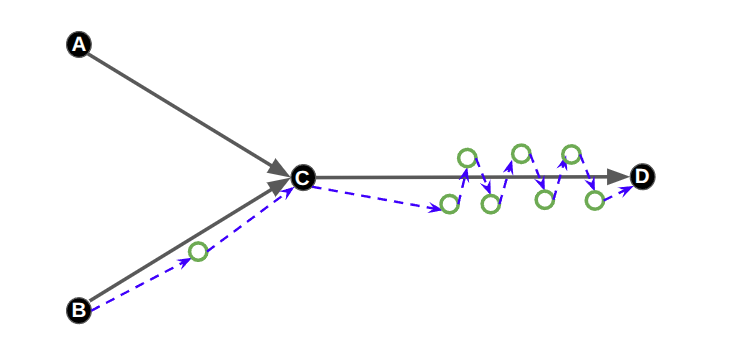
\includegraphics[width=0.9\linewidth]{figures/dynamic_nodes_edges.png}%
    }{%
      \IfFileExists{figures/dynamic_graph_overview.pdf}{%
        \includegraphics[width=0.9\linewidth]{figures/dynamic_graph_overview.pdf}%
      }{%
        \IfFileExists{figures/dynamic_graph_overview.png}{%
          \includegraphics[width=0.9\linewidth]{figures/dynamic_graph_overview.png}%
        }{\fbox{\parbox{0.88\linewidth}{\centering Dynamic graph overview figure placeholder}}}%
      }%
    }
    \caption{Dynamic, multi-relational traffic graph: static junction nodes (labeled A--D) and road edges (solid gray) with dynamic vehicle nodes (hollow green circles) and interaction edges (blue dashed).}
    \label{fig:dyn-graph}
\end{figure}

% Compact components figure: encoder, route encoder, router/MoE
\begin{figure}[t]
    \centering
    \subfloat[Graph encoder (last snapshot)]{\resizebox{0.95\columnwidth}{!}{% TikZ: Graph Encoder (GATv2 with edge features)
\tikzset{blk/.style={draw, rounded corners=2pt, thick, align=center, inner sep=5pt, fill=black!3},
 op/.style={blk, fill=blue!6}, note/.style={font=\footnotesize, align=left}}

\begin{tikzpicture}[>=Latex, node distance=8mm]
% Input features
\node[blk, minimum width=35mm] (nodes) {Node features \\ $h_v \in \mathbb{R}^d$};
\node[blk, below=of nodes, minimum width=35mm] (edges) {Edge features \\ $e_{uv} \in \mathbb{R}^{d_e}$};

% GATv2 layers
\node[op, right=12mm of nodes, minimum width=40mm] (gat1) {GATv2 Layer 1 \\ attention + aggregation};
\node[op, right=12mm of gat1, minimum width=40mm] (gat2) {GATv2 Layer 2 \\ attention + aggregation};

% Output
\node[blk, right=12mm of gat2, minimum width=35mm] (out) {Node embeddings \\ $h_v' \in \mathbb{R}^d$};

% Connections
\draw[->] (nodes) -- (gat1);
\draw[->] (edges) -- (gat1);
\draw[->] (gat1) -- (gat2);
\draw[->] (gat2) -- (out);

% Labels
\node[note, below=2mm of edges] {static graph features};
\node[note, below=2mm of out] {encoded representations};

\end{tikzpicture}
}}\\[2mm]
    \subfloat[Route encoder (vehicle intent)]{\resizebox{0.95\columnwidth}{!}{% TikZ: Route Encoder (vehicle_route_left)
\tikzset{blk/.style={draw, rounded corners=2pt, thick, align=center, inner sep=5pt, fill=black!3},
 op/.style={blk, fill=green!7}, note/.style={font=\footnotesize, align=left}}

\begin{tikzpicture}[>=Latex, node distance=8mm]
\node[blk, minimum width=42mm] (seq) {route\_left: edge IDs [$e_1,\ldots,e_L$]};
\node[op, right=12mm of seq, minimum width=38mm] (emb) {Edge-ID embedding \\ vocab $\approx1294$, dim 64};
\draw[->] (seq) -- (emb);
\node[op, right=12mm of emb, minimum width=30mm] (pool) {Mean pool};
\draw[->] (emb) -- (pool);
\node[blk, right=12mm of pool, minimum width=32mm] (out) {Route vector (64-d)};
\draw[->] (pool) -- (out);
\end{tikzpicture}



}}\\[2mm]
    \subfloat[Router and Mixture-of-Experts]{\resizebox{0.95\columnwidth}{!}{% TikZ: Router + MoE (Top-k=2 over 6 experts)
\tikzset{blk/.style={draw, rounded corners=2pt, thick, align=center, inner sep=5pt, fill=black!3},
 moe/.style={blk, fill=orange!12}, op/.style={blk, fill=black!1}, note/.style={font=\footnotesize, align=left}}

\begin{tikzpicture}[>=Latex, node distance=8mm]
% Inputs
\node[blk, minimum width=40mm] (fused) {Fused vehicle vector};
\node[op, right=12mm of fused, minimum width=40mm] (router) {Router softmax (\(\tau\)) \\ Top-$k=2$};
\draw[->] (fused) -- (router);

% Load balancing label (moved above router)
\node[above=2mm of router, font=\footnotesize] {$\lambda_{lb}$ load-balancing; optional KL-to-uniform};

% Experts row (lowered to make room for top arrows)
\matrix (experts) [row sep=0mm, column sep=6mm, right=16mm of router, below=8mm of router] {
  \node[moe, minimum width=20mm] (e0) {E0}; &
  \node[moe, minimum width=20mm] (e1) {E1}; &
  \node[moe, minimum width=20mm] (e2) {E2}; &
  \node[moe, minimum width=20mm] (e3) {E3}; &
  \node[moe, minimum width=20mm] (e4) {E4}; &
  \node[moe, minimum width=20mm] (e5) {E5}; \\
};

% Routing edges (straight from router to each expert)
\foreach \x in {0,1,2,3,4,5} {
  \draw[->] (router.south) -- (e\x.north);
}

% Combine
\node[blk, below=10mm of experts] (combine) {Weighted combine};
\foreach \x in {0,1,2,3,4,5} {\draw[->] (e\x.south) -- ++(0,-4mm) -| (combine.north);}

\node[blk, right=12mm of combine, minimum width=28mm] (eta) {ETA};
\draw[->] (combine) -- (eta);
\end{tikzpicture}



}}
    \caption{Key components: (a) two-layer GATv2 with edge features; (b) route intent via edge-ID embeddings and mean pooling; (c) sparse Top-$k=2$ routing over six experts with load balancing.}
    \label{fig:components}
\end{figure}

% (Model Configuration moved after Model Architecture)

We define three relation types:
\begin{enumerate}
    \item \textbf{Road edges ($\rho=\text{road}$):} For adjacent junctions $(u,v)$ with legal direction $u\!\to\!v$, we add $(u,v)\in E_t^{(\text{road})}$, encoding static road topology.
    \item \textbf{Traversal edges ($\rho=\text{trav}$):} If vehicle $v_i^t$ occupies segment $(a,b)$, we add $(a,v_i^t)$ and $(v_i^t,b)$, linking the vehicle to its upstream and downstream junctions.
    \item \textbf{Interaction edges ($\rho=\text{inter}$):} For vehicles $v_i^t,v_j^t$ on the same segment with spacing $d_{ij}(t)\le\varepsilon$ and aligned headings, we add $(v_i^t,v_j^t)$ weighted by $\omega(d_{ij}(t)) = e^{-d_{ij}(t)/\lambda}$.
\end{enumerate}

\paragraph{Dynamic edge construction.}
In implementation, vehicles on each road segment are ordered by their normalized position along the edge. We then create a short chain per segment: a junction$\to$first-vehicle edge (type 1), vehicle$\to$vehicle links along the ordered list (type 3), and last-vehicle$\to$junction (type 2). These dynamic edges sit on top of the static road graph (type 0).

Each node and edge carries feature vectors. Nodes use 28 features per snapshot (junction/vehicle type, kinematics, temporal encodings, zone one-hot, coordinates, current-edge attributes, demand/occupancy surrogates, and junction type). Edges use 7 features (average speed, lanes one-hot, length, demand, occupancy). Average speed, demand, and occupancy are updated per snapshot from data; vehicle features at indices for current-edge demand/occupancy are filled from the corresponding edge attributes.

\paragraph{Route intent.}
In addition to graph-based relations, each vehicle node includes a feature called \texttt{vehicle\_route\_left}, which encodes the sequence of upcoming edges along its pre-computed source--destination path. Construction: for each trip we compute a static shortest path over $E^{\mathrm{road}}$ and record its ordered edge-ID list. At time $t$, we locate the vehicle's current edge within this list and take the suffix from the next edge to the destination. Indices are the canonical 0-based edge IDs shared across the dataset (vocabulary size 1{,}294). This sequence is summarized by a Route Encoder (edge-ID embedding + mean pooling) and used in fusion.

\subsection{Temporal Windowing}
ETA prediction requires reasoning over temporal dynamics. We construct a window of $H$ consecutive snapshots:
\begin{equation}
\mathcal{G}_{t-H+1:t} = \{G_\tau\}_{\tau=t-H+1}^t,
\end{equation}
where $H$ is configurable (default $H{=}30$ in our experiments, with 30-second spacing). The prediction target is the ETA of vehicles present in the final snapshot $G_t$.

\subsection{Problem Statement}
Given a temporal window of dynamic graphs $\mathcal{G}_{t-H+1:t}=\{G_{\tau}\}_{\tau=t-H+1}^{t}$, where each snapshot $G_{\tau}$ contains static junction nodes $V^{j}$, dynamic vehicle nodes $V^{v}_{\tau}$, static road edges, and time-varying interaction edges, the goal is to predict per-vehicle ETAs at the final snapshot $t^*{=}t$. Let $\mathcal{V}_t = V^{v}_{t}$ denote vehicles present at time $t$. We learn a function $f_{\theta}$ that maps
\begin{equation}
f_{\theta}\big(\mathcal{G}_{t-H+1:t},\;\texttt{route\_left}\big) \;\to\; \hat{\mathbf{y}}_t \in \mathbb{R}^{|\mathcal{V}_t|},
\end{equation}
where $\hat{\mathbf{y}}_t[i]$ is the ETA for vehicle $i\in\mathcal{V}_t$. Training minimizes mean absolute error (MAE) over vehicles present at $t$ (additional terms are described in Section~\ref{sec:loss}):
\begin{equation}
\mathcal{L}_{\text{MAE}} = \frac{1}{|\mathcal{V}_t|}\sum_{i\in\mathcal{V}_t} \big| \hat{y}_t[i] - y_t[i] \big|.
\end{equation}

\subsection{Model Architecture}
Our DSTRA-GNN (Dynamic Spatio-Temporal Route-Aware GNN) integrates spatial, temporal, and route information. See the complete architecture in Fig.~\ref{fig:temporal-moe-eta}. The main components are:

\begin{itemize}
    \item \textbf{Graph Encoder:} Each snapshot $G_t$ is processed by a multi-layer GATv2-based encoder with residual connections and edge features, producing embeddings for junction and vehicle nodes (see the encoder panel in Fig.~\ref{fig:components}).
    \item \textbf{Temporal Aggregator:} For each pre-final snapshot $\tau\in\{t{-}H{+}1,\ldots,t{-}1\}$ we take the static road-edge features (edge\_type$=0$) and build edge-wise sequences across time. A temporal module (Transformer with sinusoidal positional encodings; GRU optional) processes these sequences per edge; the temporally aggregated edge features are then projected and pooled over all static edges to a graph-level context vector (detail in Fig.~\ref{fig:transformer-detail}). This context is broadcast to all vehicles at $t^*$ for prediction. For \emph{all} temporal variants, temporal context is computed from static road edges only for $t{-}H{+}1\ldots t{-}1$, while the final snapshot $G_t$ is encoded with the appropriate spatial topology (static or full dynamic) per variant.
    \item \textbf{Vehicle Selection:} From the final snapshot $G_t$, we retain only vehicle node embeddings, as these are the prediction targets for ETA.
    \item \textbf{Route Encoder:} Each vehicle’s remaining route (\texttt{vehicle\_route\_left}) is embedded via an edge-ID lookup (vocabulary $|E^{\mathrm{road}}|{=}1{,}294$, embedding dim 64) followed by mean pooling over the variable-length sequence (see the route panel in Fig.~\ref{fig:components}). The pooled route vector is concatenated with the vehicle embedding and temporal context when route awareness is enabled.
    \item \textbf{Fusion and MoE Head:} Vehicle embeddings, enriched with route and temporal context, are fused through a feed-forward network and routed to a sparse Top-$k$ Mixture-of-Experts (MoE) head (router panel in Fig.~\ref{fig:components}), where specialized experts capture heterogeneous traffic regimes. The output is the ETA prediction for each vehicle.
\end{itemize}

% ===== TikZ Diagram of Model Architecture =====
\begin{figure*}[t]
    \centering
    \resizebox{0.80\textwidth}{!}{% TikZ diagram: Temporal MoE ETA model
% This file is included by sections/methodology.tex

% Styles used by nodes in this diagram
\tikzset{
  block/.style = {draw, rounded corners=2pt, thick, align=center, inner sep=6pt, fill=black!3},
  small/.style = {draw, rounded corners=2pt, align=center, inner sep=4pt, fill=black!3},
  op/.style    = {block, fill=blue!6},
  opt/.style   = {block, fill=green!7},
  moe/.style   = {block, fill=orange!12}
}

\begin{tikzpicture}[>=Latex, node distance=12mm]

% --- Snapshots as an overlapped deck (shared encoder) ---
\node[block, minimum width=40mm, minimum height=16mm] (snapdeck)
  {Snapshots $t{-}H{+}1,\ldots,t$ \\ \footnotesize Dynamic graphs ($x$, $edge\_index$, $edge\_attr$)};

% faint background cards behind the main one (deck effect)
\begin{scope}[on background layer]
  % soft shadow under/behind the top card (horizontal alignment)
  \node[fill=black!12, draw=none, rounded corners=2pt, minimum width=42mm, minimum height=18mm]
    at ($(snapdeck.center)+(1.2mm,0mm)$) {};
  % aligned background cards with thicker frames (exact same size as snapdeck)
  % use snapdeck's corners to draw identically sized rectangles behind it
  \draw[rounded corners=2pt, line width=1.4pt, draw=black!70, fill=white]
    ($(snapdeck.south west)+(6mm,6mm)$) rectangle ($(snapdeck.north east)+(6mm,6mm)$);
  \draw[rounded corners=2pt, line width=1.4pt, draw=black!70, fill=white]
    ($(snapdeck.south west)+(5mm,5mm)$) rectangle ($(snapdeck.north east)+(5mm,5mm)$);
  \draw[rounded corners=2pt, line width=1.4pt, draw=black!70, fill=white]
    ($(snapdeck.south west)+(4mm,4mm)$) rectangle ($(snapdeck.north east)+(4mm,4mm)$);
  \draw[rounded corners=2pt, line width=1.4pt, draw=black!70, fill=white]
    ($(snapdeck.south west)+(3mm,3mm)$) rectangle ($(snapdeck.north east)+(3mm,3mm)$);
  \draw[rounded corners=2pt, line width=1.4pt, draw=black!70, fill=white]
    ($(snapdeck.south west)+(2mm,2mm)$) rectangle ($(snapdeck.north east)+(2mm,2mm)$);
  \draw[rounded corners=2pt, line width=1.4pt, draw=black!70, fill=white]
    ($(snapdeck.south west)+(1mm,1mm)$)  rectangle ($(snapdeck.north east)+(1mm,1mm)$);
\end{scope}

% --- Single Graph Encoder (shared across time) ---
\node[op, below=of snapdeck, minimum width=45mm] (encoder)
  {Graph Encoder \\ \footnotesize (shared across snapshots)};

% --- Temporal module (predict-on-last in impl) ---
\node[op, below=15mm of encoder, minimum width=60mm] (temp)
  {Temporal module GRU \\ \footnotesize predict at last $t^*$ };

% --- Vehicle selection ---
\node[small, below=of temp] (vehsel) {Select vehicle nodes at $t^*$};

% --- Route encoder (optional, Full) ---
\node[opt, right=20mm of vehsel, align=left, minimum width=55mm] (routeenc)
  {Route Encoder\\ \footnotesize edge-id embedding + mean pooling\\
   \footnotesize inputs: $vehicle\_route\_left$, $vehicle\_route\_left\_splits$};

% --- Fusion / Router / Experts / Output ---
\node[op,   below=of vehsel,  minimum width=70mm] (fusion)  {Fusion MLP};
\node[moe,  below=of fusion,  minimum width=70mm] (router)  {Router (softmax, temperature, noise) \\ Top-$k$ selection};
\node[moe,  below=of router,  minimum width=70mm] (experts) {Experts (Residual MLPs) $\times E$, weighted by Top-$k$};
\node[block,below=of experts, minimum width=70mm] (pred)    {Per-vehicle ETA at $t^*$};

% --- Connections ---
\draw[->] (snapdeck) -- (encoder);
\draw[->] (encoder) -- (temp);
\draw[->] (temp) -- (vehsel);
\draw[->] (vehsel) -- (fusion);
\draw[->] (fusion) -- (router);
\draw[->] (router) -- (experts);
\draw[->] (experts) -- (pred);

% optional route path (Full)
\draw[->, dashed] (vehsel) -- (routeenc);
\draw[->, dashed] (routeenc.south) |- (fusion.east);

% small notes (optional)
% \node[above=0mm of snapdeck, font=\footnotesize] {Input from sliding window dataset};
% \node[right=2mm of pred,  font=\footnotesize, align=left] {target inverted to seconds for metrics};

\end{tikzpicture}
}
    \caption{DSTRA-GNN architecture. A window of $T{=}30$ dynamic graph snapshots (shown as an overlapped deck) is processed by a \emph{shared} Graph Encoder; prediction is made at the last snapshot $t^*$. In the Full variant, a Route Encoder summarizes each vehicle's remaining path before Fusion and a Top-$k$ MoE head produces per-vehicle ETA.}
    \label{fig:temporal-moe-eta}
\end{figure*}

\begin{figure}[t]
    \centering
    \resizebox{\linewidth}{!}{% TikZ: Temporal Transformer detail (edge-level sequences)
\tikzset{blk/.style={draw, rounded corners=2pt, thick, align=center, inner sep=4pt, fill=black!3},
 mod/.style={blk, fill=blue!6}, note/.style={font=\footnotesize, align=left}}

\begin{tikzpicture}[>=Latex, node distance=6mm]
% Input sequences per static edge
\node[blk, minimum width=30mm] (e1) {$x_{e_1}^{0..H-2}$};
\node[blk, below=of e1, minimum width=30mm] (e2) {$x_{e_2}^{0..H-2}$};
\node[blk, below=of e2, minimum width=30mm] (e3) {$x_{e_3}^{0..H-2}$};
\node[note, right=2mm of e1] {edge features over time};

% Positional encodings and projection
\node[mod, right=18mm of e2, minimum width=36mm] (proj) {Input proj + \newline sinusoidal PE};
\draw[->] (e1) -- (proj);
\draw[->] (e2) -- (proj);
\draw[->] (e3) -- (proj);

% Transformer encoder stack
\node[mod, right=18mm of proj, minimum width=40mm] (tf) {Transformer Encoder \newline ($N$ layers, $n_{head}$)};
\draw[->] (proj) -- (tf);

% Take last token, norm, project back
\node[mod, right=18mm of tf, minimum width=40mm] (last) {Last token + LayerNorm};
\node[mod, below=of last, minimum width=40mm] (outp) {Output proj (to edge dim)};
\draw[->] (tf) -- (last);
\draw[->] (last) -- (outp);

% Edge-context pooling
\node[blk, right=18mm of outp, minimum width=36mm] (pool) {Mean over edges \newline Graph context};
\draw[->] (outp) -- (pool);

\end{tikzpicture}




}
    \caption{Temporal Transformer detail: per-edge sequences across $H{-}1$ snapshots are projected, positionally encoded, encoded by a Transformer stack, reduced via last-token + norm, projected back to edge dimension, then pooled over edges.}
    \label{fig:transformer-detail}
\end{figure}

\subsection{Model Configuration}
Unless stated otherwise, experiments use the following settings:
\begin{itemize}
    \item \textbf{Node/edge features}: 28 node features; 7 edge features. Temporal window $H{=}30$ consecutive snapshots.
    \item \textbf{Graph encoder}: 2-layer GATv2 with edge features, hidden size 128, 4 heads per layer, GELU activations, LayerNorm residuals, dropout 0.1.
    \item \textbf{Temporal module}: static-road edge sequences over the first $H{-}1$ snapshots. Default is a Transformer Encoder with $n_\text{head}{=}4$, $n_\text{layers}{=}2$, GELU, FFN size $2d$, dropout 0.1, and sinusoidal positional encodings; an optional single-layer GRU (hidden 128) is also supported. Aggregated edge context is projected, mean-pooled over static edges to a graph vector, then broadcast to vehicles.
    \item \textbf{Route encoder}: edge-ID embedding of size 64 with mean pooling over \texttt{vehicle\_route\_left} (vocabulary size 1294).
    \item \textbf{Fusion}: MLP  (256 hidden with GELU, LayerNorm, dropout 0.1) to a 192-dim fused representation.
    \item \textbf{MoE head}: Top-$k{=}2$ sparse routing over $6$ experts (dropout 0.1). Predictions are made for vehicles in the last snapshot only.
    \item \textbf{Target normalization}: we train in the $y_{log,z}$ space:
    \begin{equation}
    y_{log} = \log\big(1 + y_{sec}\big)
    \end{equation}
    \begin{equation}
    y_{log,z} = \frac{y_{log} - \mu}{\sigma}
    \end{equation}
    where $y_{sec}$ is the raw ETA in seconds, and $(\mu,\sigma)$ are computed on the training set; metrics are reported after inverting to seconds.
    \item \textbf{Training}: AdamW (lr $10^{-3}$, weight decay $10^{-2}$), linear warmup then cosine annealing ($T_{\text{max}}{=}200$), batch size 2, 200 epochs. Primary loss in target space with metrics reported after inversion to seconds.
    \item \textbf{Router regularization}: load-balancing weight $\lambda_\text{lb}{=}0.05$ plus optional KL-to-uniform router regularization with weight 0.002.
\end{itemize}
\subsection{Loss Functions and Training Protocol}\label{sec:loss}
We train the model with supervised regression on ETA targets using mean absolute error (MAE) in seconds:
\begin{equation}
\mathcal{L}_{\text{MAE}} = \frac{1}{N}\sum_{i=1}^N \big| \hat{y}_i - y_i \big|,
\end{equation}
where $\hat{y}_i$ and $y_i$ are the predicted and true ETAs. Additional evaluation metrics include RMSE and mean absolute percentage error (MAPE). The optimization objective includes MoE load balancing and optional router regularization:
For completeness, we report the following definitions used in evaluation:
\begin{equation}
\mathrm{RMSE} = \sqrt{\frac{1}{N}\sum_{i=1}^{N} (\hat{y}_i - y_i)^2}
\end{equation}
\begin{equation}
\mathrm{MAPE}(\%) = 100\cdot \frac{1}{N}\sum_{i=1}^{N} \left|\frac{\hat{y}_i - y_i}{y_i}\right|
\end{equation}
All metrics are computed in seconds (after inverting any target-space transforms) and averaged over vehicles in the test split.
\begin{equation}
\mathcal{L} = \mathcal{L}_{\text{reg}} + \lambda_{\text{lb}}\,\mathcal{L}_{\text{lb}} \;\; (\text{and optionally } 
\lambda_{\text{kl}}\,\mathrm{KL}(p\,\Vert\,\text{Uniform})),
\end{equation}
where $\mathcal{L}_{\text{lb}}$ encourages uniform expert usage via importance/load terms from the router, and $p$ are routing probabilities. Training occurs in a chosen target space (e.g., $y_{\text{log}}$ or $y_{\text{log\_z}}$), while metrics are reported after consistent inversion to seconds.

\paragraph{Complexity and inference.}
Per-snapshot spatial encoding is $\mathcal{O}(|E_t|)$; temporal aggregation is $\mathcal{O}(|E_\text{road}|\cdot(H{-}1))$ over static road edges only. Inference processes a window and emits per-vehicle ETAs at $t^*$ with negligible overhead beyond a single forward pass of the encoder plus temporal aggregator.

The dataset spans four simulated weeks of traffic. We partition this chronologically into two weeks for training, one week for validation, and one week for testing. This split ensures that models are evaluated on non-overlapping time intervals that include different traffic patterns (rush hours, weekends, and long trips).

% (Ablation variants are described in Experiments; removed from Methodology per structure)
